\documentclass[../main.tex]{subfiles}

\begin{document}
	\section{Diskussion und Ausblick}

	Weiterführende Möglichkeiten des Projektes bestehen. Unter anderem stehen Optionen offen, wie alle Logdateien als CSV zu exportieren um diese weiterzuverarbeiten.
	\\ \\
	Grössere weiterführende Projekte sind unter anderem ein Erkennungssystem für die Fische und die gesamte Umwelt im Tank. \\
	Folgende Punkte können zukünftig implementiert werden:
	\begin{itemize}
		\item Anzahl und Gewicht der Fische erkennen.
		\item Durch das Gewicht und die Anzahl die Fütterungsrate festlegen.
		\item Sauerstoffgehalt des Wassers erkennen und angezeigt werden. Damit man im Notfall jederzeit eingreifen kann.
		\item Gesundheit der Fische überwachen unter anderem:
		\begin{itemize}
			\item Körper und Flossenkonditionen des Fisches durch Kameras überwachen
			\item Schuppenprobleme, Deformierungen, Kiemenverfärbungen erkennen und frühzeitig warnen
		\end{itemize}
	\end{itemize}	
	Diese Punkte würden Bildbearbeitungsmethoden benötigen, welche diese Punkte erkennen können. Damit Massnahmen in den verschiedenen Fällen getroffen werden können. 
	\par 
	\begin{figure}[H]
		\centering
		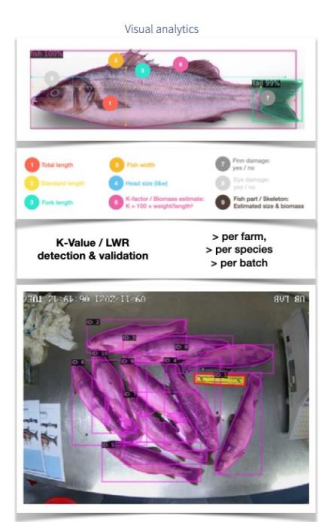
\includegraphics{../images/Imageprocessing} 
		\caption{Bildbearbeitungsmethoden}
		\label{fig:Imageprocessing}
	\end{figure}
	
	\par \noindent
	Hiermit werden weitere Möglichkeiten für Überwachungen eröffnet wie z.B:
	
	\begin{itemize}
	 	\item Verhalten 
	 	\item Sterblichkeit
	 	\item Platzgebrauch
	 	\item Gruppierungen
	 	\item Isolationen
	 	\item Schwimmgeschwindigkeit
	 	\item Körpergleichgewicht
	\end{itemize}
\noindent
	Das würde bereits Videobearbeitung erfordern, um das Verhalten auf gewisse Aktionen zu erkennen. 
	
\end{document}